\documentclass{article}%
\usepackage[T1]{fontenc}%
\usepackage[utf8]{inputenc}%
\usepackage{lmodern}%
\usepackage{textcomp}%
\usepackage{lastpage}%
\usepackage{authblk}%
\usepackage{graphicx}%
%
\title{LRP{-}6 is a coreceptor for multiple fibrogenic signaling pathways in pericytes and myofibroblasts that are inhibited by DKK{-}1}%
\author{Angela Dennis}%
\affil{Department of Cancer Biology and,}%
\date{01{-}01{-}2013}%
%
\begin{document}%
\normalsize%
\maketitle%
\section{Abstract}%
\label{sec:Abstract}%
Email a question about Dr. Salinas research on immune signaling to scientists by email.\newline%
Who is Dr. Salinas? Her main focus is on modifying immune signaling for research purposes, but she hopes to find similar methods and drugs to attack our own immune system and help researchers make groundbreaking discoveries.\newline%
Bio:\newline%
Dr. Salinas is co{-}director of the UC San Diego Chemistry Department. She is a member of the Herbstein Laboratory, an independent institute of biology and chemistry located in Suite 300 of the UCSD Bloomberg Business School. She is currently an assistant professor in the Department of Chemistry. Her research focuses on monoclonal antibodies, therapeutic targets that stimulate plasma signaling in cells, and immuno{-}oncology, which is the process of enhancing the bodys ability to fight pathogens.\newline%
Bio info:\newline%
She holds a PhD in immunology from the University of Massachusetts Boston. She has also earned a postdoctoral appointment at Johns Hopkins University, and is a senior scientist at the Institute for Systems Biology in Seattle. She recently initiated her research collaboration with MIT researchers to investigate the links between our innate immune system and antibody production in laboratory mice.\newline%
For more information about Dr. Salinas, please visit www.DrSalinas.com or contact the UCSD Chemistry Department at 949{-}496{-}5713.

%
\subsection{Image Analysis}%
\label{subsec:ImageAnalysis}%


\begin{figure}[h!]%
\centering%
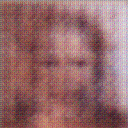
\includegraphics[width=150px]{500_fake_images/samples_5_70.png}%
\caption{A Close Up Of A Black And White Cat On The Ground}%
\end{figure}

%
\end{document}